%% FEUP THESIS STYLE for LaTeX2e
%% how to use feupteses (English version)
%%
%% FEUP, JCL & JCF, 31 July 2012
%%
%% PLEASE send improvements to jlopes at fe.up.pt and to jcf at fe.up.pt
%%

%%========================================
%% Commands: pdflatex tese
%%           bibtex tese
%%           makeindex tese (only if creating an index) 
%%           pdflatex tese
%% Alternative:
%%          latexmk -pdf tese.tex
%%========================================

\documentclass[11pt,a4paper,twoside,openright]{report}

%% For iso-8859-1 (latin1), comment next line and uncomment the second line
\usepackage[utf8]{inputenc}
%\usepackage[latin1]{inputenc}

%% English version

%% MIEIC options
%\usepackage[mieic]{feupteses}
\usepackage[mieic,juri, backrefs]{feupteses}
%\usepackage[mieic,final]{feupteses}
%\usepackage[mieic,final,onpaper]{feupteses}

%% Additional options for feupteses.sty: 
%% - onpaper: links are not shown (for paper versions)
%% - backrefs: include back references from bibliography to citation place

%% Uncomment the next lines if side by side graphics used
%\usepackage[lofdepth,lotdepth]{subfig}
%\usepackage{graphicx}
%\usepackage{float}

%% Include color package
\usepackage{color}
\definecolor{cloudwhite}{cmyk}{0,0,0,0.025}

%% Include source-code listings package
\usepackage{listings}
\definecolor{listinggray}{gray}{0.9}
\definecolor{lbcolor}{rgb}{0.9,0.9,0.9}
\lstset{
	backgroundcolor=\color{lbcolor},
	tabsize=4,    
	%   rulecolor=,
	language=[GNU]C++,
	basicstyle=\scriptsize,
	upquote=true,
	aboveskip={1.5\baselineskip},
	columns=fixed,
	showstringspaces=false,
	extendedchars=false,
	breaklines=true,
	frame=single,
	numbers=left,
	showtabs=false,
	showspaces=false,
	showstringspaces=false,
	identifierstyle=\ttfamily,
	keywordstyle=\color[rgb]{0,0,1},
	commentstyle=\color[rgb]{0,0.8,0},
	stringstyle=\color[rgb]{0.627,0.126,0.941},
	numberstyle=\color[rgb]{0.205, 0.142, 0.73},
	%        \lstdefinestyle{C++}{language=C++,style=numbers}’.
}

%% Uncomment to create an index (at the end of the document)
%\makeindex

%% Path to the figures directory
%% TIP: use folder ``figures'' to keep all your figures
\graphicspath{{figures/}}

%%----------------------------------------
%% TIP: if you want to define more macros, use an external file to keep them
%some macro definitions

% format
\newcommand{\class}[1]{{\normalfont\slshape #1\/}}

% entities
\newcommand{\Feup}{Faculdade de Engenharia da Universidade do Porto}

\newcommand{\svg}{\class{SVG}}
\newcommand{\scada}{\class{SCADA}}
\newcommand{\scadadms}{\class{SCADA/DMS}}

\usepackage{xr}
\usepackage{url}
\usepackage{hyperref}
\usepackage{nicefrac}
\usepackage{lipsum}

%%----------------------------------------

%%========================================
%% Start of document
%%========================================
\begin{document}

%%----------------------------------------
%% Information about the work
%%----------------------------------------
\title{Autotuning Parallel Application in Heterogeneous Systems}
\author{João Alberto Trigo de Bordalo Morais}

%% Uncomment next line for date of submission
\thesisdate{February 10, 2017}

%%Uncomment next line for copyright text if used
\copyrightnotice{João Bordalo, 2017}

\supervisor{Supervisor}{Jorge Manuel Gomes Barbosa}

%% Uncomment next line if necessary
%\supervisor{Second Supervisor}{Name of the Supervisor}

%% Uncomment committee stuff in the final version if used
%\committeetext{Approved in oral examination by the committee:}
%\committeemember{Chair}{Doctor Name of the President}
%\committeemember{External Examiner}{Doctor Name of the Examiner}
%\committeemember{Supervisor}{Doctor Name of the Supervisor}
%\signature

%% Specify cover logo (in folder ``figures'')
\logo{uporto-feup.pdf}

%% Uncomment next line for additional text  below the author's name (front page)
\additionalfronttext{Dissertation's preparation}

%%----------------------------------------
%% Preliminary materials
%%----------------------------------------

% remove unnecssary \include{} commands
\begin{Prolog}
  \chapter*{Abstract}

Nowadays computational platforms have been evolving to the high computational power direction, however it requires a lot of energy to achieve such high performance with single but powerful processing unit.
To manage this energy cost and keep with high performance, computers are built under the assumption of heterogeneous systems, in other words, computers that have different kind of processing units with different functions, such as CPU, GPU, Xeon Phi and FPGA. 
So, developers should take advantage of parallel activity and scheduling tasks by using the various parts of the heterogeneous systems.

Now the problem is how to efficiently achieve the highest performance possible when running software applications by taking the most advantage of such heterogeneous systems and keeping the energy cost at the minimum level without jeopardizing the application performance and its results. 
Overall, the problem consists in the coexistence work of multicore specs, its parallelism and its shared cache problems; CPU and GPU parallelism and scheduling tasks; performance; and energy costs.

For this problem's solution is expected to find/create an autotuner, or at least a concept proof, that can achieve the best performance in a software application by enhancing the application's code automatically in a level that takes the best benefit of the available hardware without elevated energy costs. To do so, after creating its code, the developer runs the autotuner and it will enhance, automatically, the code to get the best performance.

This kind of solution requires some validation process and metrics to make sure that it is doing its work and with proper results. To do so, the idea of the process' validation is going to be about comparing the behaviour of three different codes: a version of  a serialized code; a version of the same code but with an expert manually paralleling it; and a version of the serialized code but automatically parallelized. The metrics that will be used to compare these three code versions are the following: processing power; execution time; number of memory accesses; and energy consuming. 

With this solution, applications will achieve its highest performance possible in an automatic way and developers will have less burdened about creating parallel code, consequently, saving them time.

\chapter*{Resumo}

Atualmente as plataformas computacionais têm vindo a evoluir na direção do elevado poder computacional, no entanto, estas requerem uma quantidade enorme de energia para atingir elevado desempenho individualmente.
De modo a gerir este custo energético e manter a elevada performance, os computadores são construídos sobre a assunção de sistemas heterogéneos, isto é, computadores compostos por diferentes tipos de unidades de processamentos com diferentes funcionalidades, como por exemplo, CPU,GPU, Xeon Phi e FPGA.
É neste sentido que os programadores devem tirar proveito de atividade paralela e escalonamento de tarefas recorrendo às várias partes que compõem o sistema heterogéneo.

O problema incide sobre como atingir de forma eficiente o maior desempenho possível quando se corre uma aplicação de software, tirando o maior proveito dos sistemas heterogéneos e mantendo o nível de custo energético o mais baixo possível sem prejudicar o resultado e o desempenho da aplicação.

Para solucionar este problema é esperado encontrar/criar um autotuner, ou pelo menos uma prova de conceito, que consegue atingir o melhor desempenho numa aplicação de software, aprimorando automaticamente o código da aplicação a um nível que take o melhor proveito do hardware disponível sem custos elevados de energia. Para tal, após o código criado, o programador correrá o autotuner e este irá aprimorar, automaticamente, o código para atingir o melhor desempenho.

Este tipo de solução requer um processo de validação e métricas para assegurar que se está a fazer o trabalho corretamente e com resultados aceitáveis. Para tal, a ideia da validação do processo consiste em comparar o comportamento de três diferentes códigos: uma versão sequencial de um código; a versão deste mesmo código mas paralelizada por um perito; e a versão do código sequencial mas paralelizado automaticamente. As métricas que serão utilizadas para comprar estas três versões de código são as seguintes: poder de processamento; tempo de execução; número de acessos a memória; e custo energético.

Com esta solução, as aplicações conseguiram atingir o seu melhor desempenho possível de forma automática e sobrecarregando menos os programadores a criarem código paralelo o que, consequentemente, poupar-lhes-á tempo.


 % the abstract
 % \chapter*{Acknowledgements}

This dissertation is a milestone in my academic career. I have been fortunate learn theories and concepts which would have been impossible if I had not extensively carried out the needed research. I am grateful to a number of people who have guided and supported me throughout the research process and provided assistance for my venture, both technically and emotionally.

I would like to divide these acknowledgements in two parts: firstly, I would like to mention those who helped me, directly or indirectly, in terms of technical assistance and knowledge, expertise, advices and guidance during the development of this dissertation. And the other part is related to those who guided me and made never give up and maintaining focused until the end.

Beginning with the first part, and the most important person during the development of my dissertation, my supervisor, Pofessor Jorge Barbosa, who guided me in selecting the final theme for this research. My advisor was there throughout my preparation of the proposal and the conceptualization of its structure. I would not have been able to do the research and achieve learning in the same manner without his help and support. His recommendations and instructions have enabled me to assemble and finish the dissertation effectively. Additionally, He, also, gave me the opportunity to collaborate in \textit{Antarex} project, a n European project that «proposes a holistic approach capable of controlling all the decision layers in order to implement a self-adaptive application optimized for energy efficiency.»

I would also like to thank all the people from the laboratory where I performed my experiences and collaborated in Antarex's project, such as Professor João cardoso, João Bispo, Hamid Arabnejad, Tiago Carvalho, Luís Reis, Nuno Paulino, Ricardo Nobre and Pedro Pinto. They made my integration in this project much easier and helped me the best way they could and any time i asked.

A special thanks to Kremlin team, in the name of Saturnino Garcia, always ready to answer my questions and requests related to the Kremlin software.

For the second part, I would like to thank again my supervisor, Professor Jorge Barbosa, who accompanied me until the end of this process and did not allow me to give up, even in the most frustrating and dire moments.

I would also like to thank all my instructors and teachers, from the beginning of my education until the end of this fase, who throughout my educational career have supported and encouraged me to believe in my abilities. They have directed me through various situations, allowing me to reach this accomplishment.

Along side with my instructors and teacher, I would like to mention my friends from  my year's course: João Pereira, Henrique Ferrolho, João Soares, Maria Marques, José Paulo, Leonardo Faria, Pedro Castro, Rita Ferreira, Jorge Teixeira, Maria Miranda, José Cardoso, Sofia Reis, Pedro França, Gabriel Souto, David Azevedo, Pedro Faria, Vitor Teixeira and João Almeida, Sara Reis, who accompained me through this five years in university and without them it would a lot harder. The lessons learned, good and bad moments are a part of me, like this dissertation.

I would also like to specially thank more friends from my course, such as Simão Felgueiras, Francisca Paupério, Vitor Esteves, João Leal, Daniel Nunes, Cristiano Seabra,  Gonçalo Moreno, Filipe Reis, Eduarda Cunha, Daniela João, Carolina Azevedo, Mariana Silva, João Carvalho, Catarina Correia, Sofia Silva, António Ramadas, Sérgio Domingues,  Tiago Frutado, Diogo Vaz, Gustavo Silva, João Almeida, Beatriz Baldaia, Daniel Machado and João Monteiro, who, in some way, helped, guided, given me advices and lived with me during these five years in university.


I would like to mention mu friends form my birth place an elementary school who now-a-days I still make contact: Rik Rodrigues, Hugo Fernandes, Simão Teixiera, Rita Pinto, Rita Franco, Maria Silva, Catarina Cadilha, Sara Carvalho, Daniela Peixoto, Tiago Cunha, João Novo, Francisca Painhas, Ana Teixeira, Windy Noro and Guilherme Polónia, who still mean a lot to me and are always present when I need.

A special thanks to Rui Castro and Nino Rocha who were always so comprehensive, supportive and helpful every time i needed.

Finally, my mother, Maria Bordalo Morais, my father, Alberto Morais, my brothers, André and Pedro Bordalo Morais, and my grandfather, Humberto Bordalo Xavier, I would like to thank them for all the support, advices and help during all times, specially during the development of this dissertation.

In the end, to all that had supported and helped me along the course of this dissertation by giving
encouragement and providing the moral and emotional support I needed to complete my thesis.
To them, I am eternally grateful

\vspace{10mm}
\flushleft{João Bordalo}
  % the acknowledgments
  %\cleardoublepage
\thispagestyle{plain}

\vspace*{8cm}

\begin{flushright}
   \textsl{``\textbf{Katsumoto:} You believe a man can change his destiny? \\
   	\textbf{Nathan Algren:} l think a man does what he can until his destiny is revealed to him.''} \\
\vspace*{1.5cm}
           In movie: \textsl{THE LAST SAMURAI} 
\end{flushright}
       % initial quotation if desired
  \cleardoublepage
  \pdfbookmark[0]{Table of Contents}{contents}
  \tableofcontents
  \cleardoublepage
  \pdfbookmark[0]{List of Figures}{figures}
  \listoffigures
 \cleardoublepage
 \pdfbookmark[0]{List of Tables}{tables}
 \listoftables
 \chapter*{Abbreviations}
\chaptermark{ABBREVIATIONS}

\begin{flushleft}
\begin{tabular}{l p{0.8\linewidth}}
CPU			& Central Processing Unit\\
GPU			& Graphic Processing Unit\\
FPGA		& Field-Programmable Gate Array\\
OpenCL		& Open Computing Language\\
CHC			& Cooperative Heterogeneous Computing\\
OpenMP		& Open Multi-Processing\\
OS			& Operative System\\
%%%%%%%%%%%%%%%%%%%%%%%%%%%%%%%%%%%%%

WWW      & \emph{World Wide Web}
\end{tabular}
\end{flushleft}

  % the list of abbreviations used
\end{Prolog}

%%----------------------------------------
%% Body
%%----------------------------------------
\StartBody

%% TIP: use a separate file for each chapter
\chapter{Introduction} \label{chap:intro}

\section*{}
\section{Context} \label{sec:context}

Previously, computer systems were built to maximize their processing power in compactness and individually because programs were developed with a sequential approach. With the advance in microchips' technology, computers increased their processing capacity per volume, however some issues arose, such as high energy cost, high temperature and low equipment durability. To solve these issues some measures needed to take place in order to make computers systems more reliable, durable, efficient, and powerful.

Recently, the computing industry has moved away from exponential scaling of clock frequency toward chip multiprocessors in order to better manage trade-offs among performance, energy efficiency, and reliability~\cite{Datta2008}

Combining different computer processing components, such as CPU, GPU Xeon Phi and FPGA, in a single computer system removed some heavy burden in the main processing core, making the computer system with better performance and reliable. However some concerns arose: how to properly use these components without jeopardizing the computer system and application performance. Some processing components can handle specif jobs better then others and combined the computer can achieve a whole new performance level; for instance, the use of a GPU together with a CPU to accelerate deep learning algorithm, analytics, and engineering applications~\cite{NvidiaGPU}, however this kind of utility is not yet well optimized and its utility is only recently emerging.

%\section{Projeto} \label{sec:proj}

% Na continuação da secção anterior, e apenas no caso de ser um Projeto
% e não uma Dissertação, esta secção apresenta resumidamente o projeto.

% Nulla nec eros et pede vehicula aliquam. Aenean sodales pede vel
% ante. Fusce sollicitudin sodales lacus. Maecenas justo mauris,
% adipiscing vitae, ornare quis, convallis nec, eros. Etiam laoreet
% venenatis ipsum. In tellus odio, eleifend ac, ultrices vel, lobortis
% sed, nibh. Fusce nunc augue, dictum non, pulvinar sed, consectetuer
% eu, ipsum. Vivamus nec pede. Pellentesque pulvinar fringilla dolor. In
% sit amet pede. Proin orci justo, semper vel, vulputate quis, convallis
% ac, nulla. Nulla at justo. Mauris feugiat dolor. Etiam posuere
% fermentum eros. Morbi nisl ipsum, tempus id, ornare quis, mattis id,
% dolor. Aenean molestie metus suscipit dolor. Aliquam id lectus sed
% nisl lobortis rhoncus. Curabitur vitae diam sed sem aliquet
% tempus. Sed scelerisque nisi nec sem. 

\section{Motivation and Goal} \label{sec:goals}

My motivation for this thesis is to advance a little further on the field of the automatic code parallelization  and replace the manual parallelization labour because it requires a lot of time and effort to achieve significant performance.



\section{Statement of the Problem}

In the filed of achieving the highest possible performance in applications, it could be divided in for levels: hardware components level; transition between hardware and software level, the operative system level; the software level, related to the programming language; and the user level, the applications / program job, algorithms that it uses. The problem this dissertations approaches is related to the software level and the transition between hardware and software level.

Parallelizing code requires getting in touch with the programming language properties, software level, and using threads to make code paralleled, transition level between hardware and software,  since the threads handling is done by the operative system. The real problem is parallelizing code requires a lot of effort, time and knowledge because, firstly,  to apply parallelism, the target application must be analysed in order to find if it is possible to be parallelized. To do this, and if the applications uses complexed algorithms that requires expertise in other fields, such as biologic, mathematics, physics, it requires time to understand the algorithm and, then, if it has blocks that can be parallelized. Secondly, if the target programming language is suited to implement such application in order to take advantage of the parallelism. And, finally, how the parallelism is achievable with out jeopardizing applications result and performance.

In conclusion, it requires a lot of time, effort and knowledge to achieve notable impacts in applications' performance, since it is made manually.


\section{Purpose of the Work}

Applying parallel methods requires a lot because there is to many factors an variables to take in to account and this is done manually.

The purpose of this dissertation is to find patterns and what  variables makes the code parallelizable  and find what exists in the state of art, and their performance impact, that helps in achieving one step closer to the automatic parallelization. 

\section{Significance of the Work}

Making parallel code increases applications performance and, if making code paralleled  was a possible future, that would increase applications performance and. as well, increase developers performance in building applications and solutions efficiently because it would spare time and effort.

With this dissertation it is hopped that attaining automatic ways to parallelize code is achievable and prove that code being parallelized automatically is viable and trustworthy in term of performance, results and speed.


\section{Research Hypothesis}

This dissertations pretends to state that, in first place, parallelizing code is worth using and achieves grreat results in terms of performance. Secondly, automatically parallelizing code is possible and thirdly, has almost, if not, the same results as doing it manually. Additionally, this work pretends, as well, to state that Kremlin tool is an excellent starting point to make parallel code automatically. 

\section{Research Questions}

The aim of this research is to find and answer for the following questions:

\begin{itemize}
	\item Is it possible to achieve high performance level in applications in an automatic way?
	\item If so, how can it be achievable? Can it totally replace an expert?
	\item Since exists tools, like Kremlin, which help to, automatically, parallelize code, how acceptable are their results?
	\item How this specific tool can help in getting one step closer to automatic code parallelization?
	\item In which way can Kremlin be better than an expert?
\end{itemize}


\section{Dissertation's Structure} \label{sec:struct}

% Para além da introdução, esta dissertação contém mais x capítulos.
% No capítulo~\ref{chap:sota}, é descrito o estado da arte e são
% apresentados trabalhos relacionados. 
% %\todoline{Complete the document structure.}
% No capítulo~\ref{chap:chap3}, ipsum dolor sit amet, consectetuer
% adipiscing elit.
% No capítulo~\ref{chap:chap4} praesent sit amet sem. 
% No capítulo~\ref{chap:concl}  posuere, ante non tristique
% consectetuer, dui elit scelerisque augue, eu vehicula nibh nisi ac
% est. 

This dissertation is divided in seven chapters:

\begin{enumerate}
	\item \textbf{Introduction}~\ref{chap:intro}

This addresses the overall context of my dissertation, motivation and goal of the developed work, what is the problem, the purpose of the work, th impact that this work will have, the hypothesis that this research wants to prove, the questions behind the research and how this dissertation is structured.

	\item \textbf{Achieving the Highest Processing Power}~\ref{chap:sota1}
	
This chapter is the state of the art of my thesis' scope and establishes the information, knowledge and work developed so far. In this chapter there are three sections. The first section is related to the context of the state of the art in the filed. The other two sections are two different but complementary approaches which help and describe the state of the art. 	

	\item \textbf{Matrix Multiplication}~\ref{chap:sota2}
	
Still related to this dissertation state of the art, in this chapter it will presented and overview about the current state of the art for matrix multiplications, more specifically, two possible algorithms, their pseudo code, vantages and disadvantages. So, this chapter is divided in three sections: Matrix multiplication overview, Matrix multiplication generic algorithm and Matrix multiplication by line algorithm.
	
	\item \textbf{Methodology}~\ref{chap:chap4}

The Methodology chapter explains how the work will unfold, starting with the followed steps, executes experiences and what data was obtained and how this data will be analysed a validated. So, this chapter is divided in four sections: Research method, Data collection from conducted experiences, Data analysis method and Data validation.

	\item \textbf{Results and Discussion}~\ref{chap:chap5}
	
In this chapter is explained, in detail, the results obtained from all conducted experiences and the meaning and conclusions drawn from each one, the relation between them and the overall impact. So, this chapter is divided in two parts: firstly the analysis made from Kremlin's report and the comparison between Original code, Manual parallized code by an expert and Kremlin's indications to parallize code using the data from Kremlin's report.
	
	\item \textbf{Conclusion}~\ref{chap:chap6}

To sum up the work and reinforce the arguments the Conclusion chapter is divided in two sections: General conclusions and Future work. In General Conclusions section, is described the conclusion of each experiment and the overall conclusion for the experiences and the relation with the research hypothesis and the answer for the questions made. In the Future work section is presented what could be the next step and what can be done with the developed work made in this dissertation. 

	%\item References
	\item \textbf{Appendices}~\ref{ap1:general}
	
The last chapter of this dissertation, Appendices, presents, in two sections, the code developed for the conducted experiences and, for the second section, the information provided from Kremlin's report.

\end{enumerate}

 
\chapter{Achieving the Highest Processing Power} \label{chap:sota1}
%Estado da arte (escolher um nome que capte o domínio do trabalho)
%Trabalhos relacionados, tecnologias existentes, abordagens ao problema ou a problemas %semelhantes
\section*{}

The introduction describes a brief overview about each content of each chapter that this report is made up with. This chapter will focus on the state of the art in how to achieve the highest processing power. Related work and already known technologies are the main point in this chapter.  


\section{Introduction}

Following the context introduced in the previous chapter, the idea of having different processing components in a computer system doesn't improve the applications performance on its own. This is where the developers' work is crucial to take advantages of such different systems. The developers' work is to schedule the application's tasks to the different components so that these components can work simultaneously, avoiding overheads caused by their parallel activity, accessing memory at the wrong moment, memory conflicts, task dependency, wrong application's results compared with the sequential application.~\cite{Lee}

As mentioned previously, trying to create parallelized code can arise many problems and must be handled so the applications don't lose their functionalities. In order to do so, it requires a lot of time and effort to make it correctly parallelized. So trying to make code parallelization automatic is the next step in the direction of taking the most advantage of heterogeneous systems which, consequently, improves applications performance. 

This chapter is divided in two parts: one part will focus in the system's heterogeneity, how they can be used in favor of enhancing performance; and the main point of the other part is taking advantage of parallel activity by transforming sequential code into parallelized code.


\section{Using Computers' Heterogeneous Components}\label{sec:computerheterogeneous}

Technologies and frameworks in this field have been developed in order to manipulate and control efficiently the different processing components. The main goal of this technologies is to optimize application parallelization; application memory management; application workload; application scheduling queue and application kernel dimension.

An interesting fact is that the following software/frameworks that will be present are built, as its bases, under OpenCL programing language due to the fact that this language's use is targeted to heterogeneous parallel programing with CPUs and GPUs.

\subsection{OpenCL}
OpenCL is a programming language for heterogeneous parallel programing targeted to CPUs, GPUs and other processors~\cite{Shen}. In a small brief,  this language is designed to take advantage of different types of processors and facilitates heterogeneous computing integration in applications' code. The user programs in a virtual platform and the source code that has been developed there is compatible for any system that supports OpenCl. Additionally, OpenCL allows users to control the applications' tunning parallelism through its hardware abstraction. In figure~\ref{fig:opcl} there is an idea of the OpenCL plataform model and memory model for a better understanding of this hardware abstractions that was previously mentioned.

The OpenCL's programs has two parts: the compute kernels that are executed depending the number of processing  devices; and the program that will be run. The program creates a set of commands and puts them in a queue for each device, additionally, to manage the execution of each kernels, additional commands are queued in the different kernels. When the computation is finished, the result data, from the previous kernels activity, return back to the original program. 

\begin{figure}[t]
  \begin{center}
    \leavevmode
    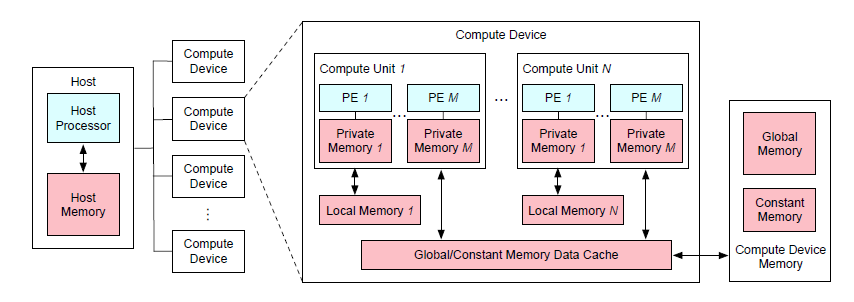
\includegraphics[width=1\textwidth]{OpenCL}
    \caption{The OpenCL platform model and the OpenCL memory model}
    \label{fig:opcl}
  \end{center}
\end{figure}

%\subsection{Cooperative Heterogeneous Computing (CHC) framework}
%~\cite{Lee}
\subsection{StarPU}
StartPU is a software tool with the purpose for programmers to use the computing power available in CPUs and GPUs, wihtout needing to care about if their programs are adapted to a specific machine and its processing components.~\cite{StartPU}
In fact, StartPU is a run-timpe support library that provides scheduling applications-provided tasks on heterogeneous environments, such as CPUs and GPUs. Additionally, it comes with programming language support, for the programming C language extensions and for OpenCL.

Programs submit computational tasks, with CPU and/or GPU implementations, and StarPU schedules these tasks and associated data transfers on available CPUs and GPUs. The data that a task manipulates are automatically transferred among accelerators and the main memory, so that programmers are freed from the scheduling issues and technical details associated with these transfers.

StarPU takes particular care of scheduling tasks efficiently, using well-known algorithms from the literature (Task Scheduling Policy). In addition, it allows scheduling experts, such as compiler or computational library developers, to implement custom scheduling policies in a portable fashion (Defining A New Scheduling Policy).
\subsection{Twin Peaks}
"Software platform that enables applications originally targeted for GPUs to be executed efficiently on multicore CPUs", mentioned by Jayanth Gummaraju, Laurent Morichetti, Michael Houston, Ben Sander, Benedict R. Gaster, Bixia Zheng, in the paper \textit{Twin peaks: a software platform for heterogeneous computing on general-purpose and graphics processors} ~\cite{Gummaraju2010}. This is a small definition of the Twin Peaks' job. The aim of this software is, firstly, to program applications using an API written in OpenCL; secondly, to compile the applications code to, for instance, add syntactic and semantic checks to make sure that the kernels meet the OpenCL requirements; and execute applications in the heterogeneous environment using CPUs and GPUs.

\section{Using Code Parallelization}\label{sec:codeparallelization}
Great advances have been made in the code parallelization. However, currently this kind of practice (the code parallelization) mostly is done by programmers and it requires a lot of effort, time and knowledge. It requires knowledge in the best practices related to what should and can't be parallelized, good knowledge on the code: its functionalities and its correct outputs because without these knowledges the chances to parallelize code correctly would be low since it is important to know if, firstly, is possible to parallelize and if, secondly, the parallelization doesn't jeopardize the programs results, outcomes and performance; to sum up, it requires time and effort to get a deep understanding of the code and to try if the code is correctly parallelized.~\cite{Jeon}

Since this practice is very costly, although grants great results at performance levels, this field has been developing ways to have results less costly, mostly in effort and time-consuming. These developments created tools to help programmers develop parallelized code, using OpenMP directives, or software tools which recommend possible parallelized regions and its theoretical speed up gain, with Kremlin, or even a way to estimate how much can a program be parallelized, with Kismet software.~\cite{Saturnino}

The following software tools that will be presented have, as its base support, OpenMP directives to help in parallelizing code, or at least, to measure performance.

\subsection{OpenMP}
OpenMP was designed to be a flexible standard, easily implemented across different platforms. the main objectives are: control structure, the data environment, synchronization, and the runtime library. 

In terms of how it really does its job, OpenMP was designed to exploit certain characteristics of shared-memory architectures. The ability to directly access memory throughout the system , combined with fast shared memory locks, makes shared-memory architectures best suited for supporting OpenMP. in practice, OpenMP is a set of compiler directives and callable runtime library routines that extend Fortran (and separately, C and C++) to express shared-memory parallelism.~\cite{Nc1998}. To be more precise, OpenMP provides standard environment variables to accompany the runtime library functions where it makes sense and to simplify  the start-up scripts for portable applications. This helps application developers who, in addition to creating portable applications, need a portable runtime environment. OpenMP has been designed to be extensible and evolve with user requirements. The OpenMP Architecture Review Board was created to provide long-term support and enhancements of the OpenMP specifications. 

\subsection{Kremlin}\label{subsec:kremlin}
The true purpose of Kremlin lies in asking the following question: "What parts of this program should I spent time parallelizing?"~\cite{ParalledSoftware}. So, in overall, Kremlin profiles a serial program and tells the programmer not only what regions should be parallelized, but also the order in which they should be parallelized to maximize the return on their effort.
Giving a non parallelized code, Kremlin guides the programmer how to achieve better performance in its program though parallelization by presenting a list of code regions that could be parallelized. this list contains a plan that will minimize the number of regions that must be parallelized to maximize the programs performance, though parallelization.

At the core of the Kremlin system is a heavyweight analysis of a sequential program’s execution that is used to create predictions
about the structure of a hypothetical, optimized parallel implementation of the program. These predictions incorporate both optimism and pessimism to create results that are surprisingly
accurate.~\cite{Garcia2011}

Overall, Kremlin is an automatic tool that, given a serial version of a program, will make recommendations to the user as to what regions (e.g. loops or functions) of the program to attack first.~\cite{Garcia2012}  

\subsection{Kismet}
Opposed to Kremlin, Kismet helps mitigate the risk of parallel software engineering by answering the question, "What is the best performance I can expect if I parallelize this program?"~\cite{ParalledSoftware}. Kismet profiles serial programs and reports the upper bound on parallel speedup based on the program's inherent parallelism and the system it will be running on.

Kismet performs dynamic program analysis on an unmodified serial version of a program to determine the amount of parallelism available in each region(e.g. loop and function) of the program. Kismet then incorporates system constrains to calculate an approximate upper bound on the program's attainable parallel speedup. ~\cite{Taylor}

In order to estimate the parallel performance of a serial program, Kismet uses a parallel execution time model. Kismet's parallel execution time model is based on the major components that affect parallel performance, including the amount of parallelism available, the serial execution time of the program, parallelization platform overheads, synchronization and memory system effects which contribute in some cases to super-linear speedups.

\section{Overview}

As mentioned before, the previously presented software tools, for both cases (using computers' heterogeneous components and using code parallelization) have their base support even being a programming language, for OpenCL, or a set of compile directives, for OpenMP. Those software tools have improved applications performance somehow, which is already good. However, looking as a software that can do everything on its own, with the minimum programmer's input, in other words, that can do things almost automatically, none of them can make it. The only software tool that is close to that automation is Kremlin because it gives what a developer should do in their code in order to increase its efficiency and performance.

Both approaches, using computers' heterogeneous components and using code parallelization, have the role to answer the state of the art premise: "achieving the highest processing power".  

\chapter{Matrix Multiplication} \label{chap:sota2}
%Estado da arte (escolher um nome que capte o domínio do trabalho)
%Trabalhos relacionados, tecnologias existentes, abordagens ao problema ou a problemas %semelhantes
\section*{}

The introduction describes a brief overview about each content of each chapter that this report is made up with. This chapter will focus on the state of the art in how to achieve the highest processing power. Related work and already known technologies are the main point in this chapter.  


\section{Introduction}


\section{Using Computers' Heterogeneous Components}\label{sec:dialecto}


\subsection{OpenCL}


\begin{figure}[t]
  \begin{center}
    \leavevmode
    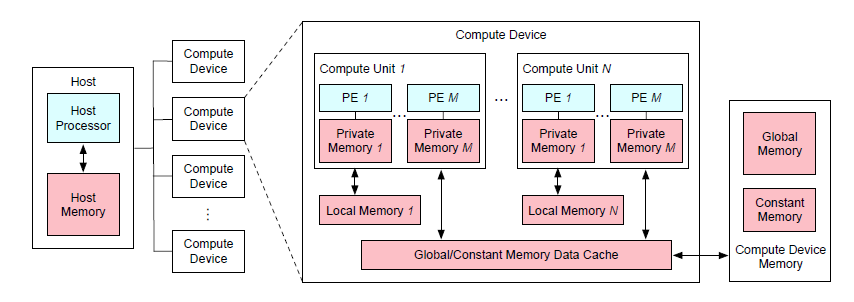
\includegraphics[width=1\textwidth]{OpenCL}
    \caption{The OpenCL platform model and the OpenCL memory model}
    \label{fig:opcl}
  \end{center}
\end{figure}



\section{Overview}

As mentioned before, the previously presented software tools, for both cases (using computers' heterogeneous components and using code parallelization) have their base support even being a programming language, for OpenCL, or a set of compile directives, for OpenMP. Those software tools have improved applications performance somehow, which is already good. However, looking as a software that can do everything on its own, with the minimum programmer's input, in other words, that can do things almost automatically, none of them can make it. The only software tool that is close to that automation is Kremlin because it gives what a developer should do in their code in order to increase its efficiency and performance.

Both approaches, using computers' heterogeneous components and using code parallelization, have the role to answer the state of the art premise: "achieving the highest processing power".  

%\chapter{How to Achieve the Highest Processing Power in a Software Application}\label{chap:chap3}

\section*{}

In this chapter is explained the problem that describes this thesis' theme, what is the solution that will be proposed, the perspective and concepts behind the proposed solution and the methodology that will be used to achieve the proposed solution and how to validate this proposed solution. 

\section{Problem}

According to the state of the art presented in the previous chapter, giving a software application, how to make it as efficiently as it is possible, in terms of performance and energy cost, without jeopardizing its results and outcome in a heterogeneous systems? 


\section{Solution's Perspective}

In order to achieve such performance in the conditions mentioned in the problem's section, I purpose an autotuner or a concept proof that will enhance the application. For that, this autotuner will receive the program's original source code and though parallel optimization a new code will emerge. This code's modification will increase applications performance without jeopardizing the application's outcome.

\subsection{Solution's Approach}

To create this autotuner, the first step is to identify what parameters exist to tune and what impact they have in the application. For this matter, with the help of Kremlin and manual expert parallelization applications will increase its performance and parameters will be found. As Kremlin detect possible parallelized code and, additionally, measures the applications speedup with such modifications, and with manual expert parallelization, there will be a confront with these results and find what is better between these two scenarios. With this confrontation, and with different use cases, the tunning parameters will be found and the autotuner will be made.

\subsection{Solution's Methodology}
\begin{figure}[t]
  \begin{center}
    \leavevmode
    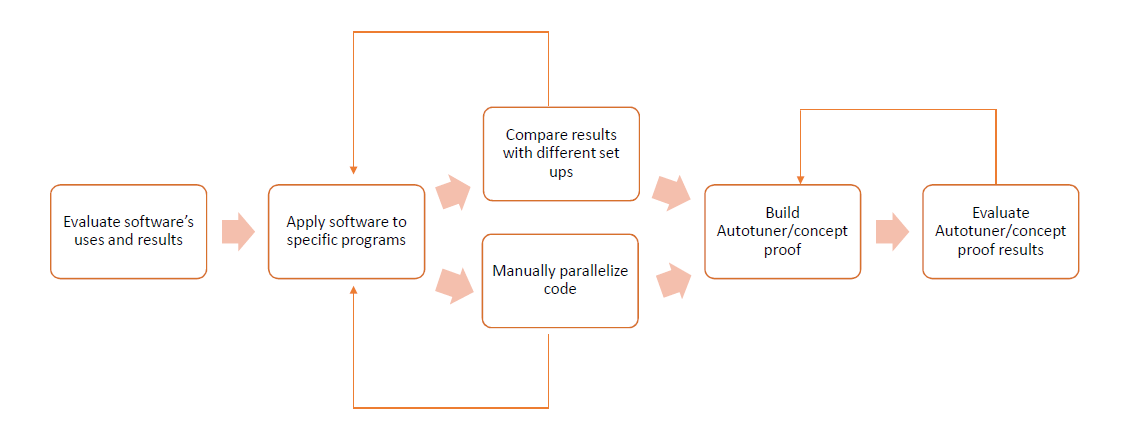
\includegraphics[width=1\textwidth]{methodology}
    \caption{Methodology that will be followed}
    \label{fig:method}
  \end{center}
\end{figure}

In the  figure ~\ref{fig:method} is outlined the steps that will be followed to create the autotuner. This methodology has six states. Firstly and using simple applications, an evaluation will be made for Kremlin to understand how to use this software tool and evaluate the results that Kremlin can achieve, for instance, if it has similar results comparing with a expert parallelizing manually the same code. Then Kremlin will be applied to specific applications. After this state, I will compare results with different Kremlin set ups and it is possible to return to the previous state to apply Kremlin but in a different configuration set up.

Simultaneously and for the same application, I will manually parallelized code in order to evaluate the results and compare with the Kremlin results. As these states (the experiences with Kremlin and the manual code parallelization) requires several attempts there will be transitions between manual and Kremlin states. 

The creations of the autotuner or concept proof happens when the tunning parameters are found after several attempts in the previous states. To make sure that the autotuner is being built correctly, evaluations will be made in order to verify the autotuner performance, so that the autotuner is correctly being made.

To sum up, this methodology as three main stages: learn and evaluate  Kremlin's uses and results; finding the tunning parameter thorough several attempts using Kremlin's outputs and manually parallelize the application's code, and compare and analyze the results in every attempt; and, in the end, the constructions of the autotuner.


\subsection{Solution's Validation}

To validate the whole methodology process, not only the autotuner itself but to compare the results between Kremlin outcomes and the code manually being parallelized, for evaluation metrics will be used: system energy consumptions when running the application; applications execution time; number of memory accesses and cache misses on the application; and the processing power measured by the number of instructions per secs. These evaluation metrics will be compared in three different cases: the original sequential code; manually paralleled code; and "automatic" paralleled code. In this last case it can be with Kremlin or with autotuner, depending in which of the methodology's state I am currently in.

To measure the above mentioned evaluation metrics, some libraries will be used: to measure energy consumptions RAPL will be used~\cite{Marcus}; to measure application  execution time OpemMP will be used ~\cite{Nc1998}; to measure number of memory accesses, cache misses and processing power PAPI ~\cite{Marcus} will be used.

Finally, two use cases will be used to validate this solution: a biopharmaceutical HPC application for accelerating drug discovery; and a self-adaptive navigation system to be used in smart cities. These use cases will be the applications that, the autotuner will try to achieve the highest processing power without jeopardizing the applications' outcome and having a low energy consumption.
%for pdis
\chapter{Methodology}\label{chap:chap4}

\section*{}



\section{Introduction}

According to the state of the art presented in chapter two, there are many means to, in some kind of automatic way, improve an applications performance. During my research, my focus was to find ways to automatically enhance the execution time in applications and programs. For this propose, Kremlin had a crucial impact in other to understand the viability of automatically parallelize code.

To study the utility and impact of automatic tools, the matrix multiplication algorithm will be used as a reference to make the performance comparison between original algorithm, an expert manually parallelizing the original algorithm and using the Kremlin's indications to parallelize the original algorithm.

To increase the credibility of this experiment, two similar algorithms for the matrix multiplication were used. As mentioned and explained in the chapter two, there is the traditional way of multiplying square matrices, naming as a quick reference \textit{Mult} algorithm, see in the appendix's list ~\ref{code:onmul} this algorithm implementation, written in C++ programming language; and the optimized algorithm that multiplies each element from the first matrix with the correspondent line of this matrix element but for the second matrix, naming this algorithm as \textit{MultLine}, see in the appendix's list ~\ref{code:onmuline} this algorithm implementation, written in C++ programming language. These algorithms differs from one another in the variables preparation and the order of the loops, which differs how the memory accessed. The \textit{MultLine} algorithm is an optimized version for matrix multiplication because it takes advantages of what is preloaded in cache and starts pre-calculating the intermediate values that will lead to the final and correct result of the multiplication, which means that won't be needed to load unnecessary values to cache memory and/or will need afterwards.  

Several experiments were conducted to understand the influence of Kremlin's indications versus code being manually parallelized  by an expert. The data's length, in this case, the matrix size; the number of threads used and if the code was parallelized were the used metrics to evaluate the results, based on a comparison of the execution time.

In this chapter it is explained the methodology and the steps followed to report in the Results and Discussion chapter the results and conclusions obtained from the performed experiences. This chapter also includes  detailed information of the acquired data from the conducted experiences, as in, how it is obtained and its meaning; also includes the methods that were used to analyse the obtained data and the reason behind those methods; and, in the end, how the data was validated in order to verify its correctness, accuracy and reliability.



\section{Research Method}

\begin{figure}[thb]
	\begin{center}
		\leavevmode
		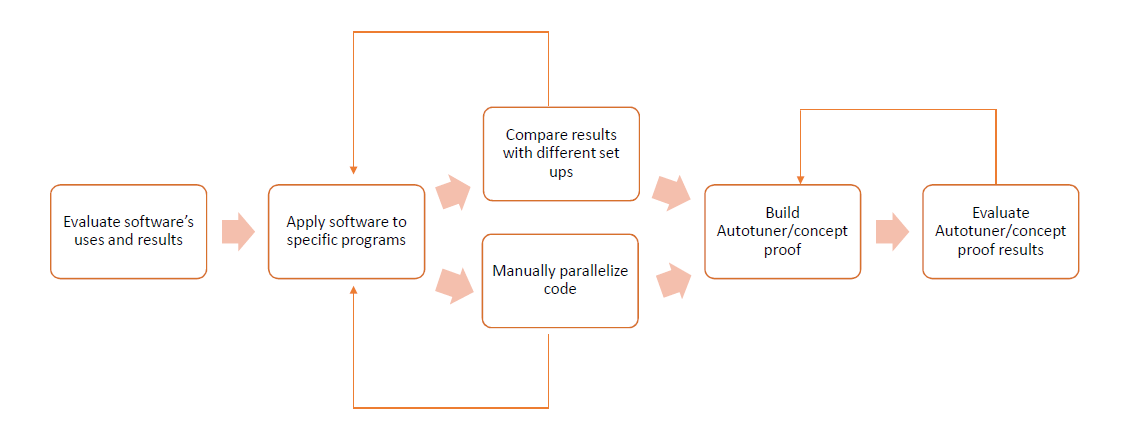
\includegraphics[width=1\textwidth]{methodology}
		\caption{Followed up methodology}
		\label{fig:workflow}
	\end{center}
\end{figure}


In Figure~\ref{fig:workflow} is outlined the steps that were followed to study the impact of the code being automaticaly parallelized. This methodology has five states. Firstly and using simple applications, an evaluation was made for Kremlin's tool in order to understand how to use this software tool and evaluate the results that it can achieve, for instance, if it has similar results comparing with an expert parallelizing manually the same code. After this, Kremlin will be applied to a set of codes with specific characteristics.

Before applying Kremlin, I manually parallelized the same sample of code in order to evaluate the results and, afterwards, compare with the Kremlin's output. Since these states (the experiences with Kremlin and the manual code parallelization) required several attempts there were transitions between these states. 

Finally, in the last state, after several attempts and tuning exercises applied to both code cases (Manual and Kremlin), data was collected from this experience to evaluate and validate its correctness in order to conclude how helpful can automatic parallelization can be.

To sum up, this methodology as three main stages: learn and evaluate  Kremlin's uses and results; finding the tuning parameter through several attempts using Kremlin's outputs and manually parallelize the application's code; and, in the end, compare and analyse the results in every attempt to take conclusions; 


\subsection{Deep learn on Kremlin's usage}

Firstly, and according to all tools/frameworks mentioned presented in the second chapter, \textit{Achieving the Highest Processing Power}, in the \textit{Using Code Parallelization} section ~\ref{sec:codeparallelization}, Kremlin was chosen because it presented the best results, easy usage and accessibility comparing to the others ~\ref{subsec:kremlin}.

Kremlin is a tool that indicates, for a sequential program, which block can be parallelised and some metrics theoretical calculated, such as, overall speedup; self parallelism for each block; the ideal time reduced for each block, in percentage; the actual time reduced for each block, in percentage; and the block coverage, in percentage. The way this tool was used is as it follows: first, an object file, \textit{*.o} extension, is required from the compilation of a sequential code. Afterwards, it is time to use the Kremlin's compiler with the generated object file so that it can profile the application. In order to do so, Kremlin's compiler runs the program as it is supposed to work. Now that the profiling is done, Kremlin generates the indications that should be followed to parallelize de provided sequential code. It also includes the blocks that can be parallelized and the impact of this theoretical parallelization with the calculations done during the profiling. Since this parallelization report is done, the developer has to interpret it, confront with the code an apply.

The Kremlin's usage seems easy, linear and fast forward, however it has some limitations that I experienced during the learning of Kremlin's capabilities: Kremlin's requires a specific environment mentioned in the Kremlin's repository ~\cite{KremlinRep}. It requires several software, libraries, compilers installations and a modern Unix operative system as its bases, such as MAC OS, RHEL 7 or other Linux distribution compatible with the software specification required. Additionally, when installing the Kremlin's tool, some minor fixes are required in order to successfully install.

From the experiences that I have been through, Kremlin has another limitation: it can not compile and profile all kind of programs: it can only profile programs that use C/C++ as its programming language; programs that take advantage of data structures from the \textit{Standard Library}, such as, stack, list, priority queue, queue, list, hash table, map, multimap, heap, and rest, since it doesn't recognize these structures; another Kremlin's limitations is its capability of compiling programs that have a deep function call level greater that seven. By deep function call level I mean the depth a function has starting from the \textit{main()} function until it is called, like a functions call tree. For instance: in a program there is the \textit{main()} function, a first level, that calls a \textit{foo1()} function, and this function calls a \textit{foo2()}, that this calls a \textit{foo3()} function, and so on. In this case, the depth of \textit{foo3()} function is four. Another small issue that Kremlin's tool has is the definition of the iterator variable used in the \textit{for}'s loops must be defined outside of the loop, as it is in C programming language.


\subsection{Kremlin's application in specific code samples}

After all the experiences made in the previous state and as mentioned in the introduction of this chapter, the matrix multiplication algorithm was used to see the potentialities of Kremlin's compiler to profile and identify the regions that can be parallelized. So, Kremlin was used in two similar, relatively similar in code structure, matrix multiplication codes. The reason behind the choice was because these two versions of the algorithm are really close to one another, which means that the testing environment is similar to one another, consequently, the results should be similar. 

\subsection{Code parallelization with Kremlin's data}

Kremlin's tool just points the regions/blocks where the program can be parallelized. In both code samples there are various numbers of inner \textit{for} loops, for the \textit{Mult} code  there are three inner \textit{for} loops, which one of them has a degree of three and the rest a degree of two; and for the \textit{MultLine} code there are four inner \textit{for} loops, which one of them has a degree of three and the rest a degree of two as well. At this time, after reading the report provided by Kremlin's tool, the developer must locate the loops, apply which loop should be parallelized, if it should be, and in case of inner \textit{for} loops, what loop should be parallelized using the OpenMP \textit{pragma} directives.

In my case, I followed all the instructions provided by Kremlin, located all the \textit{for} loops blocks indicated by kremlin's tool and applied the OpenMP \textit{pragma} directives. 

Following the two reports, ~\ref{report:onmulkremlin} ~\ref{report:onmulinekremlin}, and looking at the code's structure for both codes, it can be divided in 2 bigger parts: the \textit{for} loops used for matrices initialization and the \textit{for} loop for the matrix multiplication. With this information, understating the code and using an expert knowledge, the code parallelization was done.


\subsection{Manually Code parallelization}

In order to not be manipulated by the Kremlin's indications, the both codes were previously manually paralleliszd, this way it was guaranteed that the expert parallelization wasn't bias nor influenced.

For this parallelization, as mentioned before, it requires knowledge in, firstly, matrix multiplication algorithm; code understanding; best practice in what can and can not be parallelized, taking into account the overhead that could occur; and understand the thread behaviour in order to make it do the proper job without jeopardizing the programs outputs and/or performance.  

Analysing the code, only the \textit{for} loop for the matrix multiplication was parallelized and applied the OpenMP \textit{pragma} directives to the innermost \textit{for} loop. In this case, each code as a slight difference because for \textit{Mult} code each value of the result matrix must be calculated individually, so each thread is responsible for it and must treat that value as a private variable that isn't shared by the other threads. In the opposite, and since the \textit{MultLine} code calculates the values by adding the multiplication to the respective matrix's cell, each thread does not need to have their own private variable.

The bigger part of the code responsible for the matrices initialization wasn't parallelised, unlike in kremlin's case, because the gain would be noticeable on a large matrix size or it even could cause thread trampling, which could lead an overhead increase. 


\subsection{Results analysis}

To obtain the final execution time of each implementation (Original Matrix Multiplication ~\ref{code:onmul}, Original Matrix Multiplication by line ~\ref{code:onmuline}, Manual Matrix Multiplication by an expert ~\ref{code:onmulmanual}, Manual Matrix Multiplication by line by an expert ~\ref{code:onmulinemanual}, Kremlin Matrix Multiplication ~\ref{code:onmulkremlin} and Kremlin Matrix Multiplication by line~\ref{code:onmulinekremlin}), these six implementations suffered many modifications and tweaks since this process is a try-error until it is found the believed best parallelization. It is hardly possible to parallelize a whole program at the first try.

After compiling all these implementations and registering all the execution time for different matrix sizes and number of threads (not applied to the Original codes), this data was organized so it could be used to compare results and conclude about the performed experiences.

\section{Data collection from conducted experiences}

From all the developed work, the obtained data can be divided in two moments: Kremlin's indications reports and the execution times for the six code variations.

\subsection{Kremlin's indications reports} 

For the \textit{Mult} ~\ref{report:onmulkremlin} and \textit{MultLine} ~\ref{report:onmulinekremlin} codes were generated a report done by Kremlin. This report displays for each parallelizable block:

\begin{description}
	\item[Time reduced] percentage of time reduced if parallelization is implemented;
	\item[Ideal Time reduced] percentage of  ideal time reduced if parallelization is implemented;
	\item[Coverage] percentage of sequential execution time in a block;
	\item[Self Parallelism] amount of parallelism in a block;
	\item[Parallelism type] classification of the parallelizable block;
	\item[Loop location block] lines range of the parallelizable block;
	\item[Function location] function name of the parallelizable block, mentioning the line where the function is defined;
	\item[File location] file name of the parallelizable block, mentioning the line where the function is called;
\end{description}

The guidelines given by the report must be followed by the order it is suggested because the first detected block has the biggest impact in programs performance and should be parallelized first. The Coverage and Self Parallelism are metrics that indicates the speedup of the block, which, consequently, interferes with the time reduced. This block speedup must be equal or less then the overall program speedup, based on Amdahl's law, and can be calculated as it follows ~\cite{Saturnino}:

\begin{equation}
speedup \leq \frac{1}{(1- Coverage) - \frac{Coverage}{Self Paralelism}}
\end{equation}

\subsection{Execution times for the code variations}

After running the six implementations, the results can be divided in three major groups and each group has got the respective implementations of the \textit{Mult} and \textit{MultLine} algorithms. Each group has its own experimental environment,  with their own variables and their own meaning according to the given context.

\subsubsection{Original code}

The Original code only variable is the matrix size. This group is  a reference group to compare the results of the others groups and to quantify the impact of the others groups. The results of this group are the execution times running both matrix multiplications algorithm versions.

\subsubsection{Manual code parallelization}

The Manual code parallelization by an expert has as variables the matrix size and number of threads used for each run. This group's results are the execution times for both matrix multiplication algorithm versions. These results were used to confront with the following group in order to evaluate the improvement that a guided parallelizations, using Kremlin, can for an application.

\subsubsection{Kremlin's code parallelization}

Like the previous group, Kremlin's code parallelization indications use the same variables and provide the same type of the results. However, this group is responsible to define if it is advantageous to use software tools to help with code parallelization, in an automatic way.


\section{Data analysis method}

Analysing data is a very important stage because it is necessary to have correct conclusions. From the experiments made a lot of data as been generated and without a proper organization it is hard to understand the meaning, therefore, hard to take good conclusions from its analysis. There are three groups of code and in each group two different algorithms implementation. In order to make a correct analysis from the execution times for each situation and comparing with the others cases, the collected results were stored in tables along with the experimental related variables. Additionally, calculations were required, such as, difference between executed times between groups and algorithm implementation; ratio between these executed times; the percentage of the increase/decrease for these executed times; and the impact in the execution time that the others two groups have comparing with the Original code group. After these data manipulation, the best way to analyse all this generated and calculated data is by a dispersion plot. Using a dispersion plot, it transforms data into information visually understandable and easier to conclude because these plots display the variation of results according to the experimental environment variables.


\section{Data validation}

A considerable amount of data was generated and, more importantly, it is important that this data is scientific correct, or at least there is an explanation. In order to keep its fidelity, it is crucial to validate each and every piece of data. The first measure is to have a critical position every time by questioning if the obtained values makes sense when compared with theoretical, or expected or referenced value. In this current case, for instance, the Original group implementation is the reference, which means if the other groups have a lower execution time, or the data has some defect caused by some hardware component, or the implementation isn't good enough, or any other reason that can justify the data invalidation.

Criticism can not be the only measure because it could be luck and the gathered data happened to be correct. It is important consistency. To do so, the tests must be performed several times under the same circumstances and with a plausible and  considerable amount of values to find patterns. For this particular case  it is used a matrix size large enough, [1000,2000,3000,4000], and a wide range for the number of threads, [1,2,3,4,5,6,7,8]. For instance, if the matrix size was small, such as one hundred, the execution time would be so low and with so much error accumulated since the CPU executed fast enough that it couldn't count the time with precision. 

Finally, to make reasonable comparisons and analogies between results, the experience environments must have some connection in its variables or environment. Without a connection, the data as no meaning, therefore, it turns impossible to take conclusions. In the performed experiences, it was used the same algorithm, Matrix Multiplication, with small modifications in the implementations but with the same structure. Additionally, the environment variables were the same: number of threads and matrix size.

  


\chapter{Resultls and Discussion}\label{chap:chap5}

\section*{}
%\chapter{Conclusions and Future Work}\label{chap:chap4}

\section*{}

In this chapter is presented the conclusion of this report, including expected results and the work plan when working at this dissertation.

\section{Conclusion}
Since the beginning of \textit{Preparação da Dissertação} course, a lot has been learnt. From to develops scientific skills, such as, research from trustworthy resources, how to confirm that the resource and research is useful without wasting much time one it; to elaborate the related and formal reports and dissertations. To sum up, the first steps in the scientific field.

Many were the struggles and difficulties, but, in the end, this course is important to know where to start when working on the dissertations investigation/work.


\section{Expected Results}

What I expect from the work that will be developed during the dissertation period is the creation of an autotuner or concept proof that can achieve highest performance through available heterogeneous system components; consuming less energy compared to the old practices, like single but powerful CPUs or sequential code,  and saving programmers developing time when parallelizing code.
\section{Work Plan}
During the dissertation development, I plan the following tasks:
\begin{itemize}
    \item Learn how to use Kremlin;
    \item Apply Kremlin in an application;
    \item Result's analysis from Kremlin;
    \item Manually parallelize code on smart cities use case;
    \item Use Kremlin on smart cities use case;
    \item Compare results between manually and Kremlin;
    \item Manually parallelize code on biopharmaceutical use case;
    \item Use Kremlin on biopharmaceutical use case;
    \item Compare results between manually and Kremlin;
    \item Build autotuner /concept proof;
    \item Autotuner /concept proof result analysis;
    \item Write dissertation.
\end{itemize}

\begin{figure}[t]
  \begin{center}
    \leavevmode
    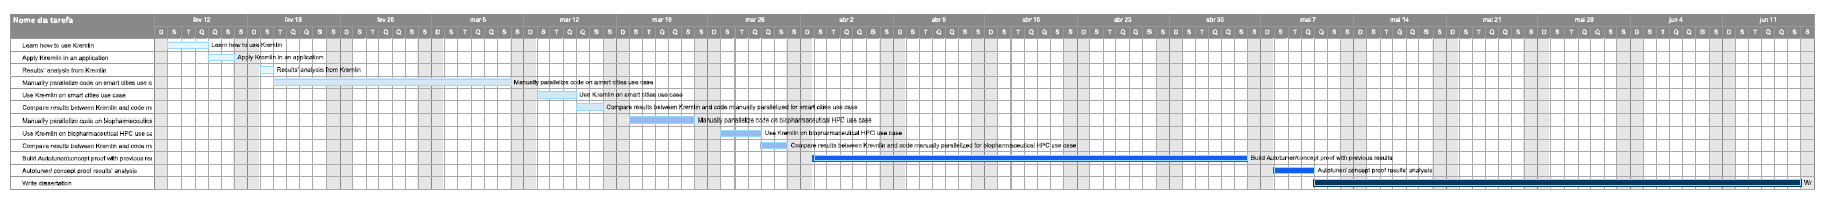
\includegraphics[width=1\textwidth]{workplan}
    \caption{Gantt's diagram for dissertation work plan}
    \label{fig:plan}
  \end{center}
\end{figure}
In figure \ref{fig:plan} is displayed the scheduling for the previous task list and their scheduled time, in the Gantt's diagram format. From previous task list, and the different choice of colors, this work plan can be divided in 5 phases: firstly, Kremlin know-how and knowledge; parallelization of the smart cities use case; parallelizations of the biopharmaceutical use case; build and validation of the autotuner; and finally, write dissertation. This work plan starts at February, thirteen, and is planned to finish at June sixteen.
%for pdis
\chapter{Conclusion}\label{chap:chap6}

\section*{}

%\chapter{Conclusões e Trabalho Futuro} \label{chap:concl}

\section*{}

Deve ser apresentado um resumo do trabalho realizado e apreciada a
satisfação dos objetivos do trabalho, uma lista de contribuições
principais do trabalho e as direções para trabalho futuro.

A escrita deste capítulo deve ser orientada para a total compreensão
do trabalho, tendo em atenção que, depois de ler o Resumo e a
Introdução, a maioria dos leitores passará à leitura deste capítulo de
conclusões e recomendações para trabalho futuro.

\section{Satisfação dos Objetivos}

Lorem ipsum dolor sit amet, consectetuer adipiscing elit. Etiam non
felis sed odio rutrum ultrices. Donec tempor dolor. Vivamus justo
neque, tempus id, ullamcorper in, pharetra non, tellus. Praesent eu
orci eu dolor congue gravida. Sed eu est. Donec pulvinar, lectus et
eleifend volutpat, diam sapien sollicitudin arcu, a sagittis libero
neque et dolor. Nam ligula. Cras tincidunt lectus quis nunc. Cras
tincidunt congue turpis. Nulla pede velit, sagittis a, faucibus vitae,
porttitor nec, ante. Nulla ut arcu. Cras eu augue at ipsum feugiat
hendrerit. Proin sed justo eu sapien eleifend elementum. Pellentesque
habitant morbi tristique senectus et netus et malesuada fames ac
turpis egestas. Vivamus quam lacus, pharetra vel, aliquam vel,
volutpat sed, nisl. 

Nullam erat est, vehicula id, tempor non, scelerisque at,
tellus. Pellentesque tincidunt, ante vehicula bibendum adipiscing,
lorem augue tempor felis, in dictum massa justo sed metus. Suspendisse
placerat, mi eget molestie sodales, tortor ante interdum dui, ac
sagittis est pede et lacus. Duis sapien. Nam ornare turpis et
magna. Etiam adipiscing adipiscing ipsum. Fusce sodales nisl a
arcu. Cras massa leo, vehicula facilisis, commodo a, molestie
faucibus, metus. Suspendisse potenti. Duis sagittis. Donec porta. Sed
urna. Maecenas eros. Vivamus erat ligula, pharetra sit amet, bibendum
et, fermentum sed, dolor. Nullam eleifend condimentum nibh. Integer
leo nibh, consequat eget, mollis et, sagittis ac, felis. Duis viverra
pede in pede. Phasellus molestie placerat leo. Praesent at tellus a
augue congue molestie. Proin sed justo eu sapien eleifend
elementum. Pellentesque habitant morbi tristique senectus et netus et
malesuada fames ac turpis egestas. 

\section{Trabalho Futuro}

Lorem ipsum dolor sit amet, consectetuer adipiscing elit. Aliquam
tempor tristique risus. Suspendisse potenti. Fusce id eros. In eu
enim. Praesent commodo leo. Nullam augue. Pellentesque tellus. Integer
pulvinar purus a dui convallis consectetuer. In adipiscing, orci vitae
lacinia semper, sapien elit posuere sem, ac euismod ipsum elit tempus
urna. Aliquam erat volutpat. Nullam suscipit augue sed
felis. Phasellus faucibus accumsan est. 

Aliquam felis justo, facilisis sit amet, bibendum ut, tempus ac,
dolor. Sed malesuada. Nunc non massa. In erat. Nulla
facilisi. Phasellus blandit, est in accumsan cursus, libero augue
elementum leo, vitae auctor mauris nisl ac tortor. Cras porttitor
ornare elit. Fusce at lorem. Sed lectus tortor, vestibulum id, varius
a, condimentum nec, lectus. Maecenas in nisi et magna pretium
aliquam. Pellentesque justo elit, feugiat nec, tincidunt a, dignissim
vel, ipsum. Sed nunc. Vestibulum ante ipsum primis in faucibus orci
luctus et ultrices posuere cubilia Curae; Aliquam tempus rhoncus
leo. Donec neque quam, cursus sit amet, ultricies varius, semper non,
pede. Donec porttitor. Sed aliquet feugiat elit.  

\vspace*{12mm}

Lorem ipsum dolor sit amet, consectetuer adipiscing elit. Phasellus
tellus pede, auctor ut, tincidunt a, consectetuer in, felis. Mauris
quis dolor et neque accumsan pellentesque. Donec dui magna,
scelerisque mattis, sagittis nec, porta quis, nulla. Vivamus quis
nisl. Etiam vitae nisl in diam vehicula viverra. Sed sollicitudin
scelerisque est. Nunc dapibus. Sed urna. Nulla gravida. Praesent
faucibus, risus ac lobortis dignissim, est tortor laoreet mauris,
dictum pellentesque nunc orci tincidunt tellus. Nullam pulvinar, leo
sed vestibulum euismod, ante ligula elementum pede, sit amet dapibus
lacus tortor ac nisl. Morbi libero. Integer sed dolor ac lectus
commodo iaculis. Donec ut odio.  
 

%%----------------------------------------
%% Final materials
%%----------------------------------------

%% Bibliography
%% Comment the next command if BibTeX file not used
%% bibliography is in ``myrefs.bib''
\PrintBib{10-myrefs}

%% comment next 2 commands if numbered appendices are not used
%\appendix
\chapter{Appendices} \label{ap1:}

\section{Developed code}


\subsection{Original Matrix Multiplication (Mult)}

\lstinputlisting[label={code:onmul},caption={Matrix Multiplication original algorithm, written in C++},firstline=217,lastline=264]{./codes/matrixmul.cpp} 

\subsection{Original Matrix Multiplication By line (MutLine)}

\lstinputlisting[label={code:onmuline},caption={Matrix Multiplication by line original algorithm, written in C++},firstline=266, lastline=316]{./codes/matrixmul.cpp}

\subsection{Manual Matrix Multiplication (Mult)}

\lstinputlisting[label={code:onmulmanual},caption={Matrix Multiplication manually parallelised using OpenMP library, written in C++},firstline=168, lastline=215]{./codes/matrixmul.cpp}

\subsection{Manual Matrix Multiplication By line (MultLine)}

\lstinputlisting[label={code:onmulinemanual},caption={Matrix Multiplication by line manually parallelised using OpenMP library, written in C++},firstline=116, lastline=166]{./codes/matrixmul.cpp}
	
\subsection{Kremlin Matrix Multiplication (Mult)}

\lstinputlisting[label={code:onmulkremlin},caption={Matrix Multiplication with Kremlin's indications for parallelization, written in C++},firstline=65, lastline=114]{./codes/matrixmul.cpp}
	
\subsection{Kremlin Matrix Multiplication By line (MultLine)}

\lstinputlisting[label={code:onmulinekremlin},caption={Matrix Multiplication by line with Kremlin's indications for parallelization, written in C++},firstline=11, lastline=63]{./codes/matrixmul.cpp}


\section{Kremlin's Reports}

\subsection{Kremlin report for Matrix Multiplication, Mult version }

\lstinputlisting[label={report:onmulkremlin},caption={Kremlin's indication of the blocks that should be parallelised and theorical variables that where calculated for Mult algorithm version},firstline=164, lastline=174]{./codes/onMultKremlin.txt}

\subsection{Kremlin report for Matrix Multiplication, MultLine version }

\lstinputlisting[label={report:onmulinekremlin},caption={Kremlin's indication of the blocks that should be parallelised and theorical variables that where calculated for MultLine algorithm version},firstline=167, lastline=181]{./codes/onMultLineKremlin.txt}




%% Index
%% Uncomment next command if index is required
%% don't forget to run ``makeindex mieic-en'' command
%\PrintIndex

\end{document}
